\documentclass[border=6pt]{standalone}
\usepackage{tikz}
\usetikzlibrary{arrows.meta,calc}
\begin{document}
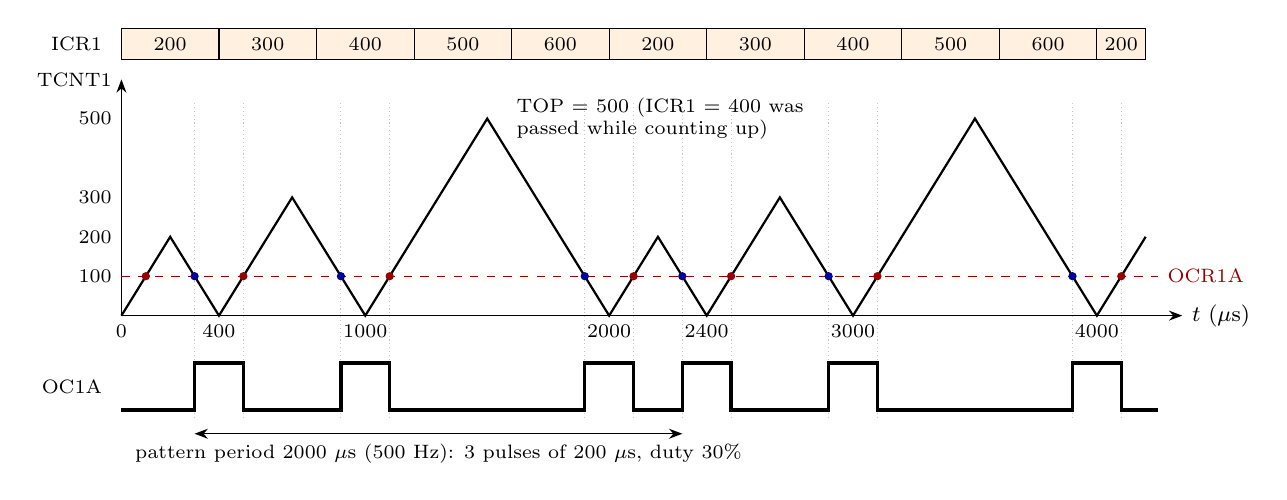
\begin{tikzpicture}[>=Stealth,font=\small,x=0.0031cm,y=1cm]
% 1 unit = 1 us (1 MHz, no prescaler). ICR1 changes every 400 us; counter simulated tick by tick:
% TOPs reached at 200 (200), 700 (300), 1500 (500); BOTTOMs at 400, 1000, 2000; pattern repeats every 2000 us
\def\s{0.005}% 1 count = 0.005 cm -> 500 counts = 2.5 cm
% ICR1 value in force
\node[anchor=east,font=\scriptsize] at (-40,3.45) {ICR1};
\foreach \a/\v in {0/200,400/300,800/400,1200/500,1600/600,2000/200,2400/300,2800/400,3200/500,3600/600,4000/200} {
  \pgfmathsetmacro{\b}{min(\a+400,4200)}
  \draw[fill=orange!12] (\a,3.25) rectangle (\b,3.65);
  \node[font=\scriptsize] at ({(\a+\b)/2},3.45) {\v};
}
\foreach \t in {300,500,900,1100,1900,2100,2300,2500,2900,3100,3900,4100} \draw[gray!45,densely dotted] (\t,-1.3) -- (\t,2.7);
\draw[->] (0,0) -- (0,3.0) node[left,font=\scriptsize]{TCNT1};
\draw[->] (0,0) -- (4350,0) node[right,font=\footnotesize]{$t$ ($\mu$s)};
\foreach \v in {100,200,300,500} \node[anchor=east,font=\scriptsize] at (0,\v*\s) {\v};
\draw[red!60!black,dashed] (0,100*\s) -- (4250,100*\s) node[right,font=\scriptsize]{OCR1A};
\draw[thick] (0,0) -- (200,200*\s) -- (400,0) -- (700,300*\s) -- (1000,0) -- (1500,500*\s) -- (2000,0)
  -- (2200,200*\s) -- (2400,0) -- (2700,300*\s) -- (3000,0) -- (3500,500*\s) -- (4000,0) -- (4200,200*\s);
\foreach \t in {100,500,1100,2100,2500,3100,4100} \fill[red!60!black] (\t,100*\s) circle (1.5pt);
\foreach \t in {300,900,1900,2300,2900,3900} \fill[blue!60!black] (\t,100*\s) circle (1.5pt);
\foreach \t in {0,400,1000,2000,2400,3000,4000} \node[below,font=\scriptsize] at (\t,0) {\t};
\node[font=\scriptsize,anchor=west,align=left] at (1580,500*\s) {TOP = 500 (ICR1 = 400 was\\passed while counting up)};
\begin{scope}[yshift=-1.2cm]
\node[anchor=east,font=\scriptsize] at (-40,0.3) {OC1A};
\draw[very thick] (0,0) -- (300,0) -- (300,0.6) -- (500,0.6) -- (500,0) -- (900,0) -- (900,0.6) -- (1100,0.6) -- (1100,0) -- (1900,0) -- (1900,0.6) -- (2100,0.6) -- (2100,0)
  -- (2300,0) -- (2300,0.6) -- (2500,0.6) -- (2500,0) -- (2900,0) -- (2900,0.6) -- (3100,0.6) -- (3100,0) -- (3900,0) -- (3900,0.6) -- (4100,0.6) -- (4100,0) -- (4250,0);
\draw[<->] (300,-0.3) -- (2300,-0.3) node[midway,below,font=\scriptsize]{pattern period 2000 $\mu$s (500 Hz): 3 pulses of 200 $\mu$s, duty 30\%};
\end{scope}
\end{tikzpicture}
\end{document}
